\documentclass[a4paper, 11pt, notitlepage, english]{article}

\usepackage{babel, textcomp}
\usepackage[latin1]{inputenc}
\usepackage[T1]{fontenc, url}
\usepackage{amsmath, amssymb}
\usepackage{amsbsy, amsfonts}
\usepackage{graphicx, color, xcolor}
\usepackage{framed, parskip}
\usepackage{flafter, caption, multicol}
\usepackage{verbatim, listings, fancyvrb}
\usepackage{mathrsfs}

\usepackage{geometry}
\geometry{headheight=0.01mm}
\geometry{top=24mm, bottom=29mm, left=39mm, right=39mm}

\renewcommand{\arraystretch}{2}
\setlength{\tabcolsep}{10pt}
\makeatletter
\renewcommand*\env@matrix[1][*\c@MaxMatrixCols c]{%
  \hskip -\arraycolsep
  \let\@ifnextchar\new@ifnextchar
  \array{#1}}


\definecolor{javared}{rgb}{0.6,0,0} % for strings
\definecolor{javagreen}{rgb}{0.25,0.5,0.35} % comments
\definecolor{javapurple}{rgb}{0.5,0,0.35} % keywords
\definecolor{javadocblue}{rgb}{0.25,0.35,0.75} % javadoc

\lstset{language=python,
basicstyle=\ttfamily\scriptsize,
keywordstyle=\color{javapurple},%\bfseries,
stringstyle=\color{javared},
commentstyle=\color{javagreen},
morecomment=[s][\color{javadocblue}]{/**}{*/},
% numbers=left,
% numberstyle=\tiny\color{black},
stepnumber=2,
numbersep=10pt,
tabsize=4,
showspaces=false,
captionpos=b,
showstringspaces=false,
frame= single,
breaklines=true}

%
% Definering av egne kommandoer og miljøer
%
\newcommand{\dd}[1]{\ \text{d}#1}
\newcommand{\f}[2]{\frac{#1}{#2}} 
\newcommand{\beq}{\begin{equation*}}
\newcommand{\eeq}{\end{equation*}}
\newcommand{\bra}[1]{\langle #1|}
\newcommand{\ket}[1]{|#1 \rangle}
\newcommand{\braket}[2]{\langle #1 | #2 \rangle}
\newcommand{\braup}[1]{\langle #1 \left|\uparrow\rangle\right.}
\newcommand{\bradown}[1]{\langle #1 \left|\downarrow\rangle\right.}
\newcommand{\av}[1]{\left| #1 \right|}
\newcommand{\op}[1]{\hat{#1}}
\newcommand{\braopket}[3]{\langle #1 | {#2} | #3 \rangle}
\newcommand{\ketbra}[2]{\ket{#1}\bra{#2}}
\newcommand{\pp}[1]{\frac{\partial}{\partial #1}}
\newcommand{\ppn}[1]{\frac{\partial^2}{\partial #1^2}}
\newcommand{\up}{\left|\uparrow\rangle\right.}
\newcommand{\upup}{\left|\uparrow\uparrow\rangle\right.}
\newcommand{\down}{\left|\downarrow\rangle\right.}
\newcommand{\downdown}{\left|\downarrow\downarrow\rangle\right.}
\newcommand{\updown}{\left|\uparrow\downarrow\rangle\right.}
\newcommand{\downup}{\left|\downarrow\uparrow\rangle\right.}
\newcommand{\bupup}{\left.\langle\uparrow\uparrow\right|}
\newcommand{\bdowndown}{\left.\langle\downarrow\downarrow\right|}
\newcommand{\bupdown}{\left.\langle\uparrow\downarrow\right|}
\newcommand{\bdownup}{\left.\langle\downarrow\uparrow\right|}
\renewcommand{\d}{{\rm d}}
\newcommand{\Res}[2]{{\rm Res}(#1;#2)}
\newcommand{\To}{\quad\Rightarrow\quad}
\newcommand{\eps}{\epsilon}
\newcommand{\inner}[2]{\langle #1 , #2 \rangle}

\usepackage{caption}

%\DeclareCaptionLabelSeparator{colon}{. }
\renewcommand{\captionfont}{\sffamily}
\renewcommand{\captionlabelfont}{\bf\sffamily}
\setlength{\captionmargin}{40pt}

\newcommand{\bt}[1]{\boldsymbol{#1}}
\newcommand{\mat}[1]{\textsf{\textbf{#1}}}
\newcommand{\I}{\boldsymbol{\mathcal{I}}}
\newcommand{\p}{\partial}
%
% Navn og tittel
%
\author{Jonas van den Brink \\ \texttt{j.v.d.brink@fys.uio.no}}
\title{MAT-INF2360 \\ Project 2}

\usepackage{titling}
\usepackage{blindtext}
\setlength{\droptitle}{6em}


\begin{document}

\vspace {2cm}
\maketitle
\vspace {2 cm}

We will be looking at a multiresolution analysis with a scaling function
$$
    \phi_{0,n} = \frac{1}{\sqrt{2}}\bigg(\frac{1}{8}\phi_{1,2n-2}+ \frac{1}{2}\phi_{1,2n-1}+\frac{3}{4}\phi_{1,2n}+\frac{1}{2}\phi_{1,2n+1}+\frac{1}{8}\phi_{1,2n+2}\bigg).
$$
We then use the notation
$\phi_{m,n} = 2^{m/2} \phi(2^m t-n)$, and let $\bt{\phi}_m = \{\phi_{m,n}\}_{n=0}^{2^mN-1}$ be a basis for the resolution spaces $V_m$.

We also define the mother wavelet as
$$\psi(t) = \frac{1}{\sqrt{2}}\phi_{1,1}(t).$$
and use the notation
$\psi_{m,n}(t) = 2^{m/2}\psi(2^m t- n), \quad \mbox{for } n=0,1,\ldots,2^m N-1$, letting 
$\bt{\psi}_m = \{\phi_{m,n}\}_{n=0}^{2^mN-1}$ be a basis for the detail spaces $W_m$.

\clearpage

\subsection*{Exercise 1)}
We will now find the change of coordinate matrix 
$P_{\bt{\phi}_1 \leftarrow \mathscr{C}_1}$, where
$$\mathscr{C}_1 = \{\phi_{0,0}, \psi_{0,0}, \phi_{0,1}, \psi_{0,1},\ldots,\phi_{0,N-1}, \psi_{0,N-1}\}.$$
This is the inverse discrete wavelet transform (IDWT)---and we will find the matrix for $N=8$.

We have
$$
\phi = \frac{1}{\sqrt{2}}\bigg(\frac{1}{8}\phi_{1,-2} + \frac{1}{2}\phi_{1,-1} + \frac{3}{4}\phi_{1,0} + \frac{1}{2}\phi_{1,1} + \frac{1}{8}\phi_{1,2}\bigg).$$
and $$\psi(t) = \frac{1}{\sqrt{2}}\phi_{1,1}(t).$$
From these we can find the first two columns of $P_{\bt{\phi}_1} \leftarrow \mathscr{C}_1$, as $N=8$, the final matrix will contain 16 rows. 
$$P_{\bt{\phi}_1 \leftarrow \mathscr{C}_1} = \frac{1}{\sqrt{2}}\begin{pmatrix}
3/4 & 0 \\
1/2 & 1 \\
1/8 & 0 \\
0 & 0 \\
\vdots & \vdots \\
0 & 0 \\
1/8 & 0 \\
1/2 & 0 
\end{pmatrix}.$$
To find the complete matrix we shift the first two columns, so that the final matrix is an MRA-matrix. 

From these two columns, we can read of the IDWT filter components $G_0$ and $G_1$, expressed in compact filter notation, these are
\begin{align*}
G_0 &= \{1/8, 1/2, \underline{3/4}, 1/2, 1/8 \}, \\
G_1 &= \{\underline{0}, 1\}.
\end{align*}


\clearpage

We now define
$$\phi^{(1)}(t) = \begin{cases}
    1+t & \mbox{if } -1 \leq t < 0, \\
    1 -t & \mbox{if } 0 \leq t < 1, \\
    0 & \mbox{otherwise}
\end{cases}.$$
It can then be shown that the scaling function we defined earlier is the convolution of this function with itself, i.e.,
$$\phi(t) = \phi^{(1)}(t)*\phi^{(1)}(t) = \int_{-\infty}^\infty \phi^{(1)}(x)\phi^{(1)}(t-x)\ \d x.$$
It can also be shown that
\begin{enumerate}
    \item $\phi$ is twice differentiable for alle $t$.
    \item $\phi$ is a third-degree polynomial on each subinterval [n, n+1].
    \item $\phi$ is 0 outside (-2,2).
    \item The functions $\{\phi(t-n)\}_{n=0}^{N-1}$ are linearily independant.
\end{enumerate}

\subsection*{Exercise 2)}
While the convolution integral that defines $\phi(t)$ is a bit tedious, it is possible to do analytically. On the next page, we show a figure that results from solving the integral numerically. The figure also shows how $\phi_{m-1,0}$ can be built up from five smaller similar functions at the level $m$.

From the figure we see that while $\phi(t)$ is not a third-degree polynomial on the whole $t\in[-2,2]$, it is equal to a third degree polynomial on each subinterval, as stated above. This means that we are looking at an MRA with piecewise third-degree polynomials.

The first resolution space $V_{0}$ is thus the space that is spanned by having a third-degree polyinomial on each subinterval $[n,n+1]$, we can write this as
$$f \in V_0 \Leftrightarrow f = \sum_{n=0}^{N-1} c_n \phi_{0,n}.$$
When we move to higher order resolution spaces, we then see that the space $V_m$ is the subspace of continuous functions where each subinterval
$$[n2^{-m},(n+1)2^{-m}],$$
are third degree polynomials.

\begin{figure}[th]
\centering
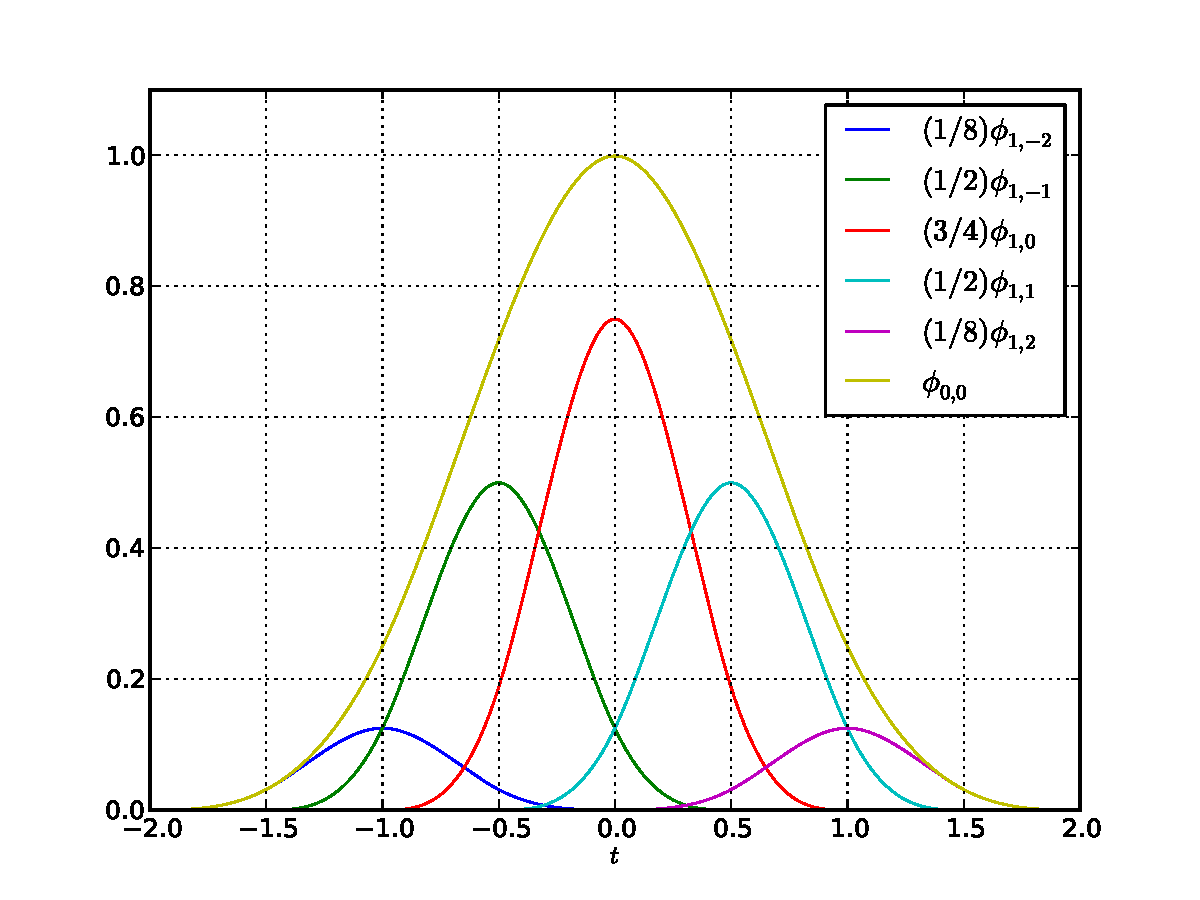
\includegraphics[width=\textwidth]{scaling_functions.pdf}
\caption{Plotting the basic scaling function, $\phi(t)$, for $t\in[-2,2]$, and showing how it can be given as the sum of $\phi_{1,k}$ for $k=-2,-1,0,1,2$.}
\end{figure}


We know that the functions $\phi_n$ are linearily independant, we have also seen that they have compact supports on $t\in[-2+n,2+n]$, meaning they have support size of four. So any sub-interval $[n,n+1]$ will have contributions from 4 different $\phi_n$. As these functions are linearily independant, they therefore effectively span the space of all third-degree polynomials, and so we see that $V_0$ contains all third-degree polynomials. From this fact alone, I would suspect our MRA to be of better accuracy when approximating functions, compared to the piecewise linear and piecewise constant functions we have looked at earlier.

However, the current mother wavelet $\psi$, (which depends on $\phi$) has no vanishing moments. Having many vanishing moments is desirable for a mother wavelet to accuractly reproduce functions. The Haar wavelet has one vanishing moment, so it might seem better than our current MRA. However, as we will see in the coming exercises, we can find a new mother wavelet that has several vanishing moments---without redefining the scaling function $\phi$. My conclusion is therefore that our MRA with the given mother wavelet might in fact be worse than the Haar wavelet. But after redefining the mother wavelet as we will do in the coming exercises, that our MRA will be better at approximating functions.


\clearpage

\subsection*{Exercise 3)}
We say that $\psi$ has $k$ vanishing moments if the integral 
        $$\int_0^N t^l \psi(t) \ \d t,$$
vanishes for $0\leq l \leq k-1$. In our case, we have seen that $\psi \geq 0$ (see figure 1), and so $\psi\geq 0$, which means that our mother wavelet has no vanishing moments.

Having a mother wavelet with many vanishing moments is very desirable, so we will now try to introduce a new mother wavelets, with four vanishing moments---we therefore define a $\hat{\psi}$ with four degrees of freedom:
$$\hat{\psi} = \psi - \alpha\phi_{0,0} - \beta\phi_{0,1}-\gamma\phi_{0,-1} - \delta\phi_{0,2}.$$
The challenge is then to decide the four real constants $\alpha$, $\beta$, $\gamma$, $\delta$ so that $\hat{\psi}$ indeed has four vanishing moments.

If $\hat{\psi}$ has four vanishing moments, we know that
$$\int\limits_0^N t^k \hat{\psi} \ \d t = \underbrace{\int\limits_0^N t^k\psi\ \d t}_{e_k} - \alpha \underbrace{\int\limits_0^N t^k\phi_{0,0}\ \d t}_{a_k} - \beta\underbrace{\int\limits_0^N t^k\phi_{0,1}\ \d t}_{b_k}-\gamma\underbrace{\int\limits_0^N t^k\phi_{0,-1}\ \d t}_{g_k} - \delta\underbrace{\int\limits_0^N t^k \phi_{0,2}\ \d t}_{d_k},$$
for $k\in{0,1,2,3}$.
This means that we have the four equations
$$a_k\alpha + b_k\beta + g_k \gamma + d_k\delta = e_k, \mbox{ for } k=0,1,2,3.$$
We can write this system of equations as the matrix equation
$$\begin{pmatrix}
a_0 & b_0 & g_0 & d_0 \\
a_1 & b_1 & g_1 & d_1 \\
a_2 & b_2 & g_2 & d_2 \\
a_3 & b_3 & g_3 & d_3 
\end{pmatrix}
\begin{pmatrix}
    \alpha \\ \beta \\ \gamma \\ \delta
\end{pmatrix} = 
\begin{pmatrix}
    e_0 \\ e_1 \\ e_2 \\ e_3
\end{pmatrix}
.
$$

\subsection*{4.)}
Let us now assume that we run an IDWT using the $G_0$ and $G_1$ filters defined in exercise 1 on the vector
$$(-\alpha,-\beta,-\delta,0,\ldots,0,-\gamma,1,0\ldots,0),$$
this vector is defined in the basis $(\bt{\phi}_0,\bt{\psi}_0)$---and so performing and IDWT gives the coordinate vector in the basis $\bt{\phi}_1$.

If we write out the vector, using the fact that it is given in the basis $(\bt{\phi}_0,\bt{\psi}_0)$, we see that it is
$$-\alpha \phi_{0,0} - \beta \phi_{0,1} - \delta  \phi_{0,2} - \gamma \phi_{0,N-1} + \psi_{0,0}.$$
As $\phi$ is periodic, we can use the equality $\phi_{0,N-1} = \phi_{0,-1}$, and then it is apparent that this coordinate vector corresponds to the function $\hat{\psi}$ in the basis $(\bt{\phi}_0,\bt{\psi}_0)$.

\clearpage

We can calculate both $\phi(t)$ and the coefficients $\alpha$, $\beta$, $\gamma$, $\delta$ analytically, giving the MRA which uses $\hat{\psi}$ as the mother wavelet and $\phi$ as the scaling function. We will not do these calculations here, as they are tedious. But the resulting digital filters are as follows
\begin{align*}
    G_0 &= \frac{1}{16}\{1,4,\underline{6},4,1\}, \\
    G_1 &= \frac{1}{128}\{5,20,1,-96,-70,\underline{280},-70,-96,1,20,5\}, \\
    H_0 &= \frac{1}{128}\{-5,20,-1,-96,70,\underline{280},70,-96,-1,20,-5\}, \\
    H_1 &= \frac{1}{16}\{1,-4,\underline{6},-4,1\}.
\end{align*}

\subsection*{Exercise 5)}

The digital filters $H_0$, $H_1$, $G_0$, $G_1$ are especially suited for lossless compression for what I assume are two reasons. First of, the filter coefficients are all dyadic fractions, which can be handled exactly in computer arithmetic---this means we get no round-off errors, which would effectively ruin lossless coding.


\subsection*{Exercise 6)}

We will now find the continiuous frequency response of the filters $G_0$ and $G_1$. 

From theorem 3.15 we know that continiuous frequency response of a filter is given by
$$\lambda_s(\omega) = \sum_k t_k e^{-ik\omega},$$
where $t_k$ are the filter coefficients.

Simply inserting the filter coefficients gives
\begin{align*}    
\lambda_{G_0}(\omega) &= \frac{1}{8}\bigg(3 + 4\cos(\omega) + \cos(2\omega)\bigg).
\\
\lambda_{G_1}(\omega) &= \frac{1}{64}\bigg(5\cos(5\omega) + 20\cos(4\omega) + \cos(3\omega) - 96\cos(2\omega) - 70\cos(\omega) + 140\bigg).
\end{align*}

On the next page we have plotted these functions. We see that $G_0$ is a low-pass filter. As $\omega$ near 0 and $2\pi$ correspond to low frequencies, while frequencies near $\pi$ correspond to high frequencies. Similarily we see that $G_1$ is a high-pass filter. This fits well with the examples of $G_0$ and $G_1$ given in the book, where they have always been a lowpass and highpass filter respectively.

\begin{figure}
    \centering
    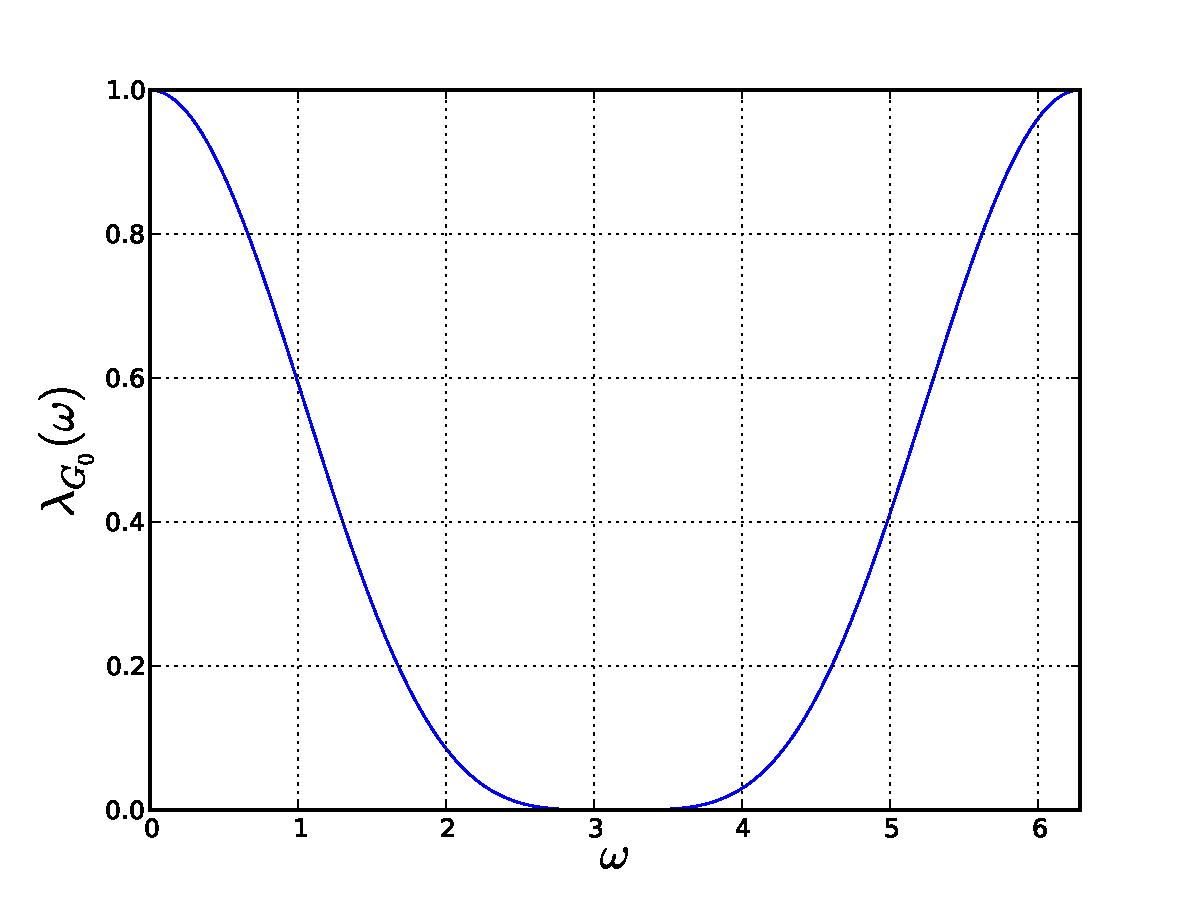
\includegraphics[width=\textwidth]{g0.pdf}
    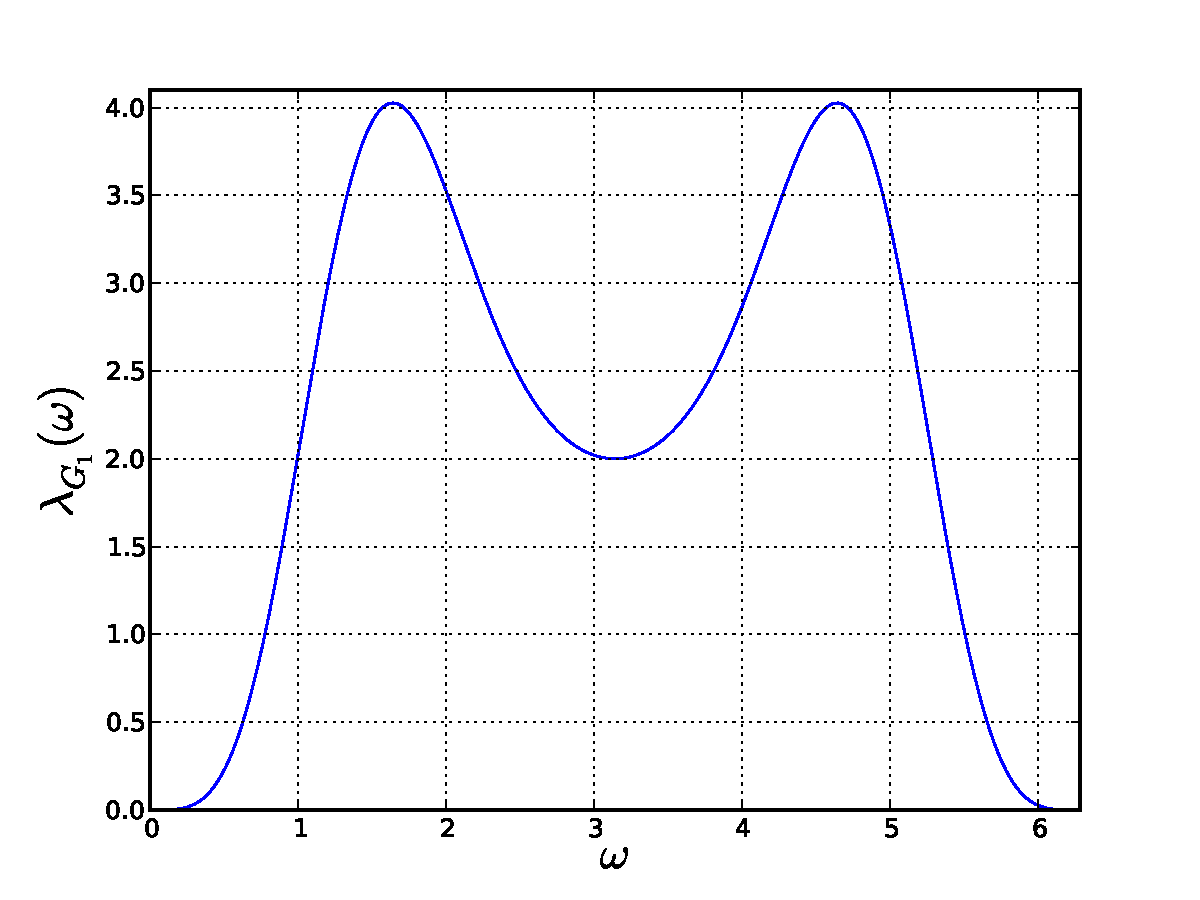
\includegraphics[width=\textwidth]{g1.pdf}
    \caption{Continiuous frequency response of the two digital filters $G_0$ and $G_1$.}
\end{figure}

\clearpage

\subsection*{Exercise 7)}
I opt not to do exercise 7 as it requries me to run code in matlab, while I prefer to stick with python---as decribed in the introduction to the assignment, it is OK to opt out of this exercise.

\subsection*{Exercise 8)}
We will now run some sound experiments on our wavelet. We use the functions \texttt{playDWTfilterslower} and \texttt{playDWTfilterslowerdifference}. Here, the first function performs an $m$-level DWT on the first $2^{17}$ sound samples of the file \verb+castanets.wav+, it then sets all the coefficients in the detail spaces to zero, and transforms the signal back into a sound using an IDWT. Meaning the first function performs lossy compression on the audio by truncating the detail. The second function takes only the truncated detail, and converts that back into a sound signal using an IDWT.

We make a simple script that plays both the compressed, truncated sound and the missing detail for $m=1,2,3,4$ for both the Haar wavelet, and the mother wavelet we have defined in this assignment. The code is as follows

\begin{lstlisting}
g0 = (1./16)*array([1,4,6,4,1])
g1 = (1./128)*array([5,20,1,-96,-70,280,-70,-96,1,20,5])
h0 = (1./128)*array([-5,20,-1,-96,70,280,70,-96,-1,20,-5])
h1 = (1./16)*array([1,-4,6,-4,1])

for m in range(1, 5):
    print "Haar wavelet, m=%i, compressed sound" % m
    playDWTlower(m)
    print "Our mother wavelet, m=%i, compressed sound" % m
    playDWTfilterslower(m,h0,h1,g0,g1)
    print "Haar wavelet, m=%i, detail information" % m
    playDWTlowerdifference(m)
    print "Our mother wavelet, m=%i, detail information" % m
    playDWTfilterslowerdifference(m,h0,h1,g0,g1)
\end{lstlisting}

When listening to the sound, we hear that for $m=1$, both wavelets make little difference to the sound, and the missing detail is of very low volume. Due to the small difference, it is hard to discern any real difference between the wavelets. For $m=2$ however, the Haar wavelet still plays a sound that sounds a lot like the original, but our wavelet has truncated a lot more of the signal. This is even more evident when listening to the missing detail, while the detail for the Haar wavelet has increased somewhat from $m=1$, the detail for our wavelet has grown a lot more, and we hear that when trucating this much detail the sound gets distored a whole lot. For $m=3$ the trucated sound of the Haar wavelet is getting quite poor, but it is still comparably better than our wavelet gave for $m=2$. The truncated sound for our wavelet for $m=3$ has very little resemblence to the original sound. We hear that the missing details of both wavelets start to sound like the original audio, which makes sense as we are effectively truncating out more and more of the original sound. For $m=4$ both truncated sounds are pretty rubbish.


\end{document}